\documentclass[twocolumn]{article}
\usepackage{PRIMEarxiv}

\usepackage[utf8]{inputenc} % allow utf-8 input
\usepackage[T1]{fontenc}    % use 8-bit T1 fonts
\usepackage{hyperref}       % hyperlinks
\usepackage{url}            % simple URL typesetting
\usepackage{booktabs}       % professional-quality tables
\usepackage{amsfonts}       % blackboard math symbols
\usepackage{amsmath}
\usepackage{amsthm}


\usepackage{natbib}

\usepackage{multirow}

\usepackage{algorithm}
\usepackage{algpseudocode}

\usepackage{nicefrac}       % compact symbols for 1/2, etc.
\usepackage{microtype}      % microtypography
\usepackage{cuted}
\usepackage{fancyhdr}       % header
\usepackage{graphicx}       % graphics
\usepackage{subfig}

\graphicspath{{images/}}     % organize your images and other figures under media/ folder

\usepackage{multicol}
\usepackage{tcolorbox}
%Header
\pagestyle{fancy}
\thispagestyle{empty}
\rhead{ \textit{ }} 

% Update your Headers here
\fancyhead[LO]{Convolution}
% \fancyhead[RE]{Firstauthor and Secondauthor} % Firstauthor et al. if more than 2 - must use \documentclass[twoside]{article}


\newtheorem*{note}{Note}
  

\newtheorem{theorem}{Theorem}
\tcolorboxenvironment{theorem}{
    colback=blue!5!white,
    boxrule = 0.2pt,
    boxsep=1pt,
    left= 2pt, right=2pt, top=2pt, bottom=2pt,
    oversize = 1.5pt,
    sharp corners, 
    before skip = \topsep,
    after skip = \topsep
}



%% Title
\title{Tensorized Pauli Composer
%%%% Cite as
%%%% Update your official citation here when published 
%\thanks{\textit{\underline{Citation}}: 
%\textbf{Authors. Title. Pages.... DOI:000000/11111.}} 
}

\author{
    \href{https://orcid.org/0000-0002-4876-7820}{
        
\includegraphics[scale=0.06]{orcid.pdf}\hspace{1mm}Hyunseong Kim}\\
  Department of Physics and Photon Science,  \\
  Gwangju Institute of Science and Technology\\
  Gwangju\\
  \texttt{qwqwhsnote@gm.gist.ac.kr} \\
  %% examples of more authors
  %% \AND
  %% Coauthor \\
  %% Affiliation \\
  %% Address \\
  %% \texttt{email} \\
  %% \And
  %% Coauthor \\
  %% Affiliation \\
  %% Address \\
  %% \texttt{email} \\
  %% \And
  %% Coauthor \\
  %% Affiliation \\
  %% Address \\
  %% \texttt{email} \\
}

\begin{document}
\twocolumn[ 
\begin{@twocolumnfalse}
    \begin{center}

    \maketitle

\begin{abstract}

%--------------------------------------------------------
In the paper, a new method was designed to construct a hamiltonian matrix 
which is given by a form of weighted summation of Pauli operators.
A symplectic representation of Pauli terms allows us to express finite dimension Hilbert space 
as a matrix form. 
Therefore, Pauli basis representation of hamiltonian could be treated as one kind of symplectic representation. 
A transformation between two specific symplectic representations was designed.
One is a common XZ code and the other is an index of Pauli basis matrix of TPD algorithm\cite{Hantzko_2024}.
With inversed TPD algorithm, the transformation of the code yields a common matrix representation from weighted Pauli summation.
The transformation between two codes consist of simple bitwise XOR operation.
Consequently, the benefit of original benefit of TPD is preserved in iTPD.
In addition to the algorithm, a term-chasing version was developed for sparse matrix in Pauli basis.
It is roughly $O(16^n)$ time complexity but, in sparse case and $<5$ qubit system, 
it showed 10 time faster than the prior algorithm.
The algorithm has $O(n4^n)$ time complexity in the worst case, 
and comparing to the term-by-term construction method with $O(n16^n) $ complexity, 
it is computationally efficient for general case.
\end{abstract}

% keywords can be removed
\keywords{Matrix composition \and Pauli polynomial \and Tensor product}
    \end{center}
\end{@twocolumnfalse}
]
\section{Introduction}
The research proposes a method to construct 
a specific Pauli basis matrix representation of weighted Pauli polynomial.
The Pauli basis matrix is a representation of finite dimension Hilbert space 
in Heisenberg representation. 
In other word, the representation is faithful to every operator in Hilbert space.
Moreover, the matrix is a result matrix of Tensorized Pauli Decomposition(\texttt{TPD}) algorithm 
which had been presented by Hantzko et al\cite{Hantzko_2024}.
Since the decomposition process was sequential basis transformation,
the inverse direction is also well-defined. 
Combining these two results yields the inversed TPD algorithm(\texttt{iTPD}),
transforming a given weighted Pauli polynomial to its single matrix representation.

\begin{equation}
    \sum_i^n \lambda_i P_i \rightarrow_{\mbox{\texttt{iTPD}}} H
\end{equation}

Following sections demonstrate a brief review of TPD algorithm, especially
index determination of single Pauli element. 
Consequently, a symplectic representation of Pauli element was introduced.
Treating the representation as \textit{p}-adic representation provides a connection between Pauli element, and matrix element.
In the last section, the inverse TPD algorithm was compared with 
the other algorithms in complexity and real execution time in hardware.

\section{Tensorized Pauli Decomposition Algorithm}

In 2024, Hantzko et al proposed that 
general $\mathbf{M}_{2^n}(\mathbb{C})$ matrices could be efficiently decomposed into 
several Pauli terms with corresponding coefficients, using a tensorized block matrix manipulation\cite{Hantzko_2024}.

\begin{equation}
    \sum_{i=0}^3 c_i \sigma_i = 
    \begin{bmatrix}
        A_{11} & A_{12}\\
        A_{21} & A_{22}
    \end{bmatrix}
    \rightarrow_{TPD}
    \begin{bmatrix}
        c_0 & c_1\\
        c_2 & c_3
    \end{bmatrix}
\end{equation}

where, 
\begin{equation}
    \label{eq:tpd_transform}
    \begin{array}{ccc}
        A_{11} & = &  c_0 + c_3\\
        A_{12} & = &  c_1 - i c_2\\
        A_{21} & = &  c_1 + i c_2\\
        A_{22} & = &  c_0 - c_3.
    \end{array}
\end{equation}

The basic idea is decoupling the coefficients of each tensor producted space, iteratively. 
See Figure \ref{fig:tpd_diagram}.
The decomposition process is non-linear in $2^n \times 2^n$ matrix space. 
However, it is a basis transformation in a higher dimension $\mathbb{C}^N$ space, 
which is isomorphic to the vector spaces with $N = 4^n$ dimension.
For example, the $2 \times 2$ dimension matrix of a 1-qubit system, the process could be expressed as 
$\mathbf{v} \in \mathbb{C}^4$. 


\begin{figure}[!h]
    \centering
    \includegraphics*{images/tpd_diagram.pdf}
    \caption{Iterative diagram of Tensorized Pauli Decomposition algorithm.}
    \label{fig:tpd_diagram}
\end{figure}

\begin{equation}
    \frac{1}{2}
    \begin{bmatrix}
        1 & 0 &  0 &  1\\
        0 & 1 &  1 &  0\\ 
        0 & i & -i &  0\\ 
        1 & 0 &  0 & -1 
    \end{bmatrix}_{TPD}
    \begin{bmatrix}
        A_{11} \\
        A_{12} \\
        A_{21} \\
        A_{22}
    \end{bmatrix} =
    \begin{bmatrix}
        c_0\\
        c_1\\
        c_2\\
        c_3
    \end{bmatrix}
\end{equation}

In $2 \times 2$ matrix with computational basis, the next matrix is a \textit{Pauli basis matrix} of 1 qubit system.

\begin{equation}
    \begin{bmatrix}
        c_0 & c_1\\
        c_2 & c_3
    \end{bmatrix}
\end{equation}

In the vectorized representation, the intermediate step of TPD algorithm 
could be represented with the next notation. 

\begin{eqnarray}
    &\begin{bmatrix}
        A_{11} \\
        A_{12} \\
        A_{21} \\
        A_{22}
    \end{bmatrix}_1 \otimes
    \begin{bmatrix}
        A_{11} \\
        A_{12} \\
        A_{21} \\
        A_{22}
    \end{bmatrix}_2 \otimes
    &\cdots \otimes
    \begin{bmatrix}
        A_{11} \\
        A_{12} \\
        A_{21} \\
        A_{22}
    \end{bmatrix}_{n-1} \otimes
    \begin{bmatrix}
        A_{11} \\
        A_{12} \\
        A_{21} \\
        A_{22}
    \end{bmatrix}
    \nonumber\\
    & &\Downarrow_{i \text{steps}, i>2} \label{eq:vec_tpd}\\
    &\begin{bmatrix}
        c_0\\
        c_1\\
        c_2\\
        c_3
    \end{bmatrix}_1 \otimes
    \begin{bmatrix}
        c_0\\
        c_1\\
        c_2\\
        c_3
    \end{bmatrix}_2 \otimes
    &\cdots \otimes
    \begin{bmatrix}
        A_{11} \\
        A_{12} \\
        A_{21} \\
        A_{22}
    \end{bmatrix}_{n-1} \otimes
    \begin{bmatrix}
        A_{11} \\
        A_{12} \\
        A_{21} \\
        A_{22}
    \end{bmatrix}_n\nonumber
\end{eqnarray}

For the $n$-fold matrix, the researcher can choose the basis transformation, freely.
The transformation even permits the different basis in each product and each sub-matrix
operations. 
In original implementation, each Pauli term was chased during the process. 
Therefore, they mapped the coefficients by adding a character to each string variables 
in each step of the iteration. 
The result Pauli basis matrix has identical coefficients without considering indexing.
By choosing appropriate basis transformation, the decomposition yields the Latin matrix whose element indexes are XZ symplectic representation
of Pauli terms in Reggio et al\cite{reggio_fast_2023}.
In below sections, the index of the Pauli basis matrix as \textit{ij-index}.

\section{Symplectic representation of Pauli element}

A generalized Pauli matrix is defined with a sequential tensor product of 
$2\times 2$ Pauli matrices.

\begin{equation}
    P = (i)^m \otimes_j^n \sigma_j
\end{equation}

From Pauli matrices, $\{\sigma_0, \sigma_1, \sigma_2, \sigma_3\}$, replacing $\sigma'_2$ into $\sigma_2$, where $\sigma_2 = i \sigma'_2$,
and separating phase to the outside yield
a tensor product representation of $n$-fold Pauli element has a next form.

\begin{equation}
    P_{g} = \{\sigma_0 , \sigma_1, \sigma'_2, \sigma_3\}
\end{equation}

\begin{equation}
    P = (i)^m \otimes_j^n \sigma_j
\end{equation}

where, $m$ is a number of occurrence of $\sigma'_2$ in the product.
Since $\sigma'_2 = \sigma_1 \sigma_3$ holds true, we can decompose the given $n$-fold Pauli term as next two
parts; elements of families, $X, Z$. 
The example families are $z$-family and $x$-family referred by Reggio et al\cite{reggio_fast_2023}.

\begin{equation}
    \label{eq:xz_decompose}
    \otimes_j^n \sigma_j = \left( \otimes_{j \in \{0, 1\}}^n \sigma_j \right) \left( \otimes_{k \in \{0, 3\}}^n \sigma_k \right)
\end{equation}

Eq(\ref{eq:xz_decompose}) yields a unique binary vector tuple representation of length 2, replacing
 $I \rightarrow 0, X, Z \rightarrow =1$ in each memeber.

\begin{equation}
    P = (\vec{z}, \vec{x}), \, \vec{z}, \vec{x} \in \{0, 1\}^N
\end{equation}

where $\vec{z}, \vec{x}$ are binary vector representation of $\otimes_{j \in \{0, 1\}}^n \sigma_j, \otimes_{j \in \{0, 3\}}^n \sigma_j$ indicates $I=0, X=1, Z=1$.

A 2-adic representation of binary vector permit them to be treated with 
a single integer tuple, $(n_z, n_x)$, ignoring phase factor.

\begin{align}
    \dots110 \leftrightarrow \cdots + 1*2^2+1*2^1+0*2^0\\
    P \leftrightarrow (n_z, n_x)\label{eq:symplectic_nznx}
\end{align}

For example, $(6, 5)$ of 3-qubit system is a symplectic representation of $\text{YXI}$.

\begin{equation}
    \begin{array}{c}
        6 = 1 \cdot 2^2 +1 \cdot 2^1 + 0 \cdot 2^0 = X \otimes X \otimes I\\
        5 = 1 \cdot 2^2 +0 \cdot 2^1 + 1 \cdot 2^0 = Z \otimes I \otimes Z
    \end{array}
\end{equation}

Comprehensive example is, $IXXZYY$, Pauli element could be transformed to integer tuple.
\begin{align}
    IXXZYY = (-i)^f (IIIZZZ) \cdot (IXXIXX)\\
    \rightarrow (-i)^f ([0,0,0,1,1,1], [0,1,1,0,1,1]) \\
    \rightarrow (f, 7, 27)
\end{align}

This is a symplectic tuple representation of Pauli element.
If the phase term, $f$, was ignored, every Pauli elements are corresponding to 
each element of $2^n \times 2^n$ dimension matrix.


\begin{align}
    H = \lambda_0 IXX + \lambda_1 YXZ + \lambda_2 ZIX\\
    H = [H]_{n_z, n_x} \\
    = \begin{bmatrix}
        0 & 0 & 0& \lambda_0 & 0 & 0 & 0& 0\\
        0 & 0 & 0& 0 & 0 & 0 & 0& 0\\
        0 & 0 & 0& 0 & 0 & 0 & 0& 0\\
        0 & 0 & 0& 0 & 0 & 0 & 0& 0\\
        0 & \lambda_2 & 0& 0 & 0 & 0 & 0& 0\\
        0 & 0 & 0& 0 & 0 & 0 & \lambda_1& 0\\
        0 & 0 & 0& 0 & 0 & 0 & 0& 0\\
        0 & 0 & 0& 0 & 0 & 0 & 0& 0\\
    \end{bmatrix}\label{eq:Pauli basis_sym}
\end{align}

A binary vector representation is now commonly adopted in quantum computing frameworks 
such as IBM Qiskit and Pennylane written by Xanadu, 
because the representation has a significant benefit in execution time.
IBM implemented the above symplectic vector representation 
for their \textit{Pauli} class in python library, \text{Qiskit},
to use the above binary implementation\cite{Qiskit}. 
However, in the paper, the order of the symplectic representation 
is reversed order of the IBM implementation. 
There is no difference in algebra implementation and 
commutation conversion routine, however, the conversion to index of coefficient
matrix is more direct in the reversed order than the IBM order.


\subsection{TPD for symplectic representation}

Eq (\ref{eq:Pauli basis_sym}) seems a one candidate of Pauli basis matrix 
for \texttt{iTPD}. Unfortunately, it is not, but still it is a good starting point to combine with \texttt{TPD} algorithm, 
\texttt{TPD} could be modified to generate a Pauli basis matrix
whose index is a symplectic tuple of Pauli elements whose element value is a weight of the term.
See modified version code in \cite{kim_2024}\footnote{In \textit{tp} directory.}.

Unfortunately, the modified-\texttt{TPD} has less practical than 
original \texttt{TPD}.
During the calculation, in $k$-th step, additional $2^k \times 2^k$ size memory 
is required to swap the partition of the matrix, and it yields 
a great inefficient in spatial and time complexity.
Therefore, a transformation is required preserving a computational benefit of TPD algorithm
The transformation converts a symplectic tuple representation to Pauli basis.

\subsection{Symplectic tuple to Pauli basis matrix}

\begin{figure}
    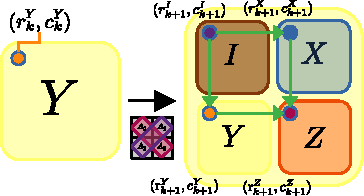
\includegraphics[width=\linewidth]{index_change_tpd.pdf}
    \caption{Index diffusion diagram by TPD decomposition process}
    \label{fig:index_change_tpd}
\end{figure}

\begin{theorem}
    \label{thm:index_conversion}
    For a given symplectic representation, $(n_x, n_z)$ of the given Paili term, $P$,
    their index, $(i, j)$, in Pauli basis matrix is determined by next formula

    \begin{equation}
        \label{eq:ij_nznx}
        (i, j) = (n_z, n_x^\wedge n_z)
    \end{equation}

    where, ${}^\wedge$ is a XOR bitwise operator. 
\end{theorem}

\begin{proof}
    From $k$-th iteration of the TPD algorithm of $2^n \times 2^n$ dim square matrix, 
    the unit sub-matrix dimension is $2^{n-k}$ and there are 4 block matrices, see Figure \ref{fig:tpd_diagram}.
    With $(n_z, n_x)$ symplectic tuple representation, 
    each $k$-th binary values of 2-adic representation of $n_z, n_x$ determine a $k+1$ index movement in Fig (\ref{fig:index_change_tpd}).

    \begin{equation}
        \begin{bmatrix}
            I& X\\
            Y & Z\\
        \end{bmatrix} = \begin{bmatrix}
            0_z \cdot 0_x & 0_z \cdot 1_x\\
            1_z \cdot 1_x & 1_z \cdot 0_x\\
        \end{bmatrix}
    \end{equation}
    
    where, $0_z, 1_z, 0_x, 1_x$ are $k$-th binary value of $(n_z, n_x)$ of Pauli element.
    Let them as $nz_k, nx_k$.

    For row index, $nz_k\in \{0, 1\}$ the Z-binary determine
    the row index movement, if $nz_k = 1$, the row location is changed by $+2^{n-k}$ else it is not.
    For column index, the column index changed by $+0$ if $(1_x, 0_z)$ or $(0_x, 1_z)$, 
    else $+2^{n-k}$ if $(0_x, 0_z)$ or $(1_x, 1_z)$.
    It is a simple XOR binary operator, thereby 
    $2^{n-k} * nz_k^{\wedge}nx_k, \, nz_k\in \{0_z, 1_z\}, nx_k \in \{0_x, 1_x\}$

    Thus, we have (i, j) coefficient index of XZ representation by iteration from 1-th to $n$-th. 
    In 2-adic representation of integer, they are identity and bitwise XOR operator of $(nz, nx)$.
    \begin{equation}
        \begin{array}{clcc}
        i =& \sum_{k=0}^{n-1} 2^{k} nz_k &=& nz\\
        j =& \sum_{k=0}^{n-1} 2^{k} nz_k^{\wedge} nx_k &=& nz^{\wedge}nx
        \end{array}
    \end{equation}

\end{proof}

Using Eq (\ref{eq:ij_nznx}), weighted Pauli polynomial could be transformed to 
a Pauli basis matrix directly applied for \texttt{iTPD}.

Theorem \ref{thm:index_conversion} provides 1-1 correspondence 
between Pauli basis matrix element location and each Pauli element.
The symplectic tuple representation is restored by next relationship.

\begin{equation}
    (nz, nx) = (i, i^\wedge j)
\end{equation}

\section{Minor improvement in TPD}

In original TPD, Pauli elements were chased in each iteration, 
by constructing each $k$-th Pauli characters of all elements.
However, with Eq (\ref{eq:ij_nznx}), the weights in Pauli basis matrix 
are directly determine corresponding Pauli elements.
Therefore, the character storing routine could be eliminated from the original TPD algorithm.

\section{iTPD algorithm}

\subsection{Naive version}

The previous section showed that TPD algorithm is a sequential 
applying of unitary transformation for each vectors in a product representation.
By the property of unitary, the inverse transformation is well-defined 
in $4^n$ dimension, and \texttt{iTPD} is defined with a $2^n \times 2^n$ space representation with 
sub-block matrix additions. 
The $\{c_i\}_{i=0}^3$ coefficients in Eq (\ref{eq:tpd_transform}) is restored as 

\begin{equation}
    \label{eq:restore}
    \begin{array}{ccc}
        A_{11} &=& c_0 + c_3\\
        A_{12} &=& c_1 + i c_2\\
        A_{21} &=& c_1 - i c_2\\
        A_{22} &=& c_0 - c_3\\
    \end{array}
\end{equation}.

The total process is achieved by iteratively applying the Eq (\ref{eq:restore}) in reverse order of \texttt{TPD} algorithm. 
The inverse process is written in Algorithm \ref{alg:naive_inverse}.
With symplectic code conversion(\texttt{SCC}) algorithm \ref{alg:ppoly_to_Pauli basis}, 
it yields \textit{Tensorized Pauli composer algorithm}(\texttt{TPC}).

\begin{algorithm}
    \caption{Symplectic code conversion}\label{alg:ppoly_to_Pauli basis}
    \begin{algorithmic}
        \Require $N \gets$ qubit number, $P \gets \sum_i \lambda_i P_i$ (weighted Pauli summation).
        \State $M \gets$ Zero matrix of dim $(N,N)$
        \For{$(\lambda_i, n_z^i, n_x^i)$ \textbf{in} $P$}
            \State $row \gets n_z^i$
            \State $col \gets {n_z^i}^\wedge n_x^i$
            \State $M[row, col] \gets \lambda_i$
        \EndFor
        \Return{$M$}
    \end{algorithmic}
\end{algorithm}


\begin{algorithm}
    \caption{Naive \texttt{iTPD}}\label{alg:naive_inverse}
    \begin{algorithmic}
        %\Require poly = $\{(c_i, (nx_i, nz_i))\}_{i=1}^k$
        %\Require n = Tensor Product dimension \Comment{Qubit number}
        %\Comment{Conversion to ij index}
        %\State polyij $\gets$ [] 
        %\For{ i \textbf{in} range(k)}
        %    \State $c_i \gets$ poly[i].c
        %    \State $nx_i \gets$ poly[i].nx
        %    \State $nz_i \gets$ poly[i].nz
        %    \State{polyij[i] $\gets (c_i, (nz_i, nx_i^\wedge nz_i))$ } 
        %\EndFor
        %\Comment{Construct Pauli basis matrix}
        %\State $M \gets $ Zero matrix of ($2^n$, $2^n$).
        %\For{c, i, j \textbf{in} polyij}
        %    \State{M$[\text{i}][\text{j}]$ = c} 
        %\EndFor
        \Require $M \gets$ Pauli basis matrix of $(2^n, 2^n)$
        \State matdim $\gets 2^n$
        \State steps $\gets$ n
        \State unit\_size $\gets$ 1

        \For{step \textbf{in} steps}
            \State step1 $\gets$ step+1
            \State mat\_size $\gets 2*\text{unit\_size}$
            \State indexes $\gets$ [matdim/$2^{\text{step1}}$]
            \State indexes\_ij $\gets$ mat\_size*indexes
            \For{i \textbf{in} indexes\_ij}
                \For{i \textbf{in} indexes\_ij}
                \State $r_{1s}\gets$ i
                \State $r_{1f2s}\gets$ $r_{1s}$ + unit\_size
                \State $c_{1s}\gets$ j
                \State $c_{1f2s}\gets$ $c_{1s}$ + unit\_size
                \State $r_{2f}\gets$ $r_{1f2s}$ + unit\_size
                \State $c_{2f}\gets$ $c_{1f2s}$ + unit\_size

                \State coef $\gets$ 1

                \State $M$[$r_{1s}$: $r_{1f2s}$, $c_{1s}$:$c_{1f2s}$] += coef*$M$[$r_{1f2s}$: $r_{2f}$, $c_{1f2s}$:$c_{2f}$]
                \State $M$[$r_{1f2s}$: $r_{2f}$, $c_{1f2s}$:$c_{2f}$] = $M$[$r_{1s}$: $r_{1f2s}$, $c_{1s}$:$c_{1f2s}$] -2*coef *$M$[$r_{1f2s}$: $r_{2f}$, $c_{1f2s}$:$c_{2f}$]

                \State coef $\gets - \sqrt{-1}$ 
                \State $M$[$r_{1f2s}$: $r_{2f}$, $c_{1s}$:$c_{1f2s}$] += coef*$M$[$r_{1s}$: $r_{1f2s}$, $c_{1f2s}$:$c_{2f}$]
                \State $M$[$r_{1s}$: $r_{1f2s}$, $c_{1f2s}$:$c_{2f}$] = $M$[$r_{1f2s}$: $r_{2f}$, $c_{1s}$:$c_{1f2s}$] -2*coef *$M$[$r_{1s}$: $r_{1f2s}$, $c_{1f2s}$:$c_{2f}$]
                
                \EndFor
            \EndFor
            \State unit\_size $\gets$ 2*unit\_size
        \EndFor
        \Return{$M$}
    \end{algorithmic}
\end{algorithm}

\begin{algorithm}
    \caption{TPC}\label{alg:TPC}
    \begin{algorithmic}
        \Require $N \gets$ qubit number, $P \gets \sum_i \lambda_i P_i$
        \State $M \gets$ \texttt{SCC}($N, P$)%\ref{alg:ppoly_to_Pauli basis} ($N$, $P$)
        \State $H \gets$ \texttt{iTPD}($M$)%\ref{alg:naive_inverse}
        \Return{$H$}
    \end{algorithmic}
\end{algorithm}

The algorithm is a combination of \texttt{iTPD} and the above symplectic construction
method. If Pauli elements are stored in string type, the conversion requires 
some computational resources, but if a framework store them as symplectic code,
it is very efficient to convert the representation. 
This approach is already adopted in some frameworks\cite{dion2024efficientlymanipulatingpaulistrings}\cite{kim_opttrot}.
In addition, as has mentioned in \cite{Hantzko_2024}, it does not need further 
instant matrix to save the terms, so that spatial complexity of the algorithm is also practical 
in large system.

\subsection{Effective term chasing}

During the calculation, if two partial matrices were zero matrix, then 
the calculation is meaningless. This case arises in sparse Pauli basis matrix; 
Hamiltonian has few Pauli terms.
In sparse case, chasing non-zero term provides some benefit in calculation time.

If we know an index set of Pauli terms, where their coefficients are not zero,
we could avoid the operation for zero sub matrices terms in the intermediate steps of the composition.
The non-zero terms are denoted with \textit{effective} terms. 
Considering I-Z and X-Y calculation, when $k$ number of Pauli terms were given, 
there is a $k_{eff}$ number of effective terms where

\begin{equation}
    k = k_{eff} + d,\, d \geq 0
\end{equation}, $d$ is a number of the duplicated terms.

From the $i$-th effective index set, the effective index set for the next step is calculated by
quotient of 2, such as 

\begin{equation}
    \label{eq:term_chasing}
    \begin{array}{ccc}
        row_{i+1}&=& r_i \\
        col_{i+1}&=& c_i
    \end{array}
\end{equation}

where, $row_i = 2*m_i + r_i$ and $col_i = 2*n_i + c_i$.
The $k_i$ number is same with $(k_{eff})_{i-1}$ number. 

For example, in $2^4 \times 2^4$ Pauli basis matrix, 
if we have 
(1, 14), 
(2, 13), 
(3, 1), 
(6, 4),
(7, 4),
(7, 5),
(13, 9),
(14, 10) elements 
were non-empty Pauli terms. 
We can chase the non-empty unit indexes with Eq (\ref{eq:term_chasing})

\begin{equation}
    \begin{array}{lccccc}
                & (1, 14)     & (0, 7)   &  (0, 3)& (0,1)&(0,0)\\
                & (2, 13)     & (1, 6)   &  (0, 0)& (0,0)&\\
                & (3, 1)      & (1, 0)   &  (1, 1)& (1,1)&\\
                & (6, 4)      & (3, 2)   &  (3, 2)& -    &\\
                & (7, 4)      & (6, 4)   &  -     & -    &\\
                & (7, 5)      & (7, 5)   &  -     & -    &\\
                & (13, 9)     & -        &  -     & -    &\\
                & (14, 10)    & -        &  -     & -    &\\
       k        & 8           & 6        &  4     & 3    & 1\\
       k_{eff}  & 6           & 4        &  3     & 2    & 1
    \end{array}
\end{equation}.

See \ref{alg:effective_terms} for further details.

%See details in appendix 2. %Computational details.

\begin{algorithm}
    \caption{Effective term chasing \texttt{iTPD}}\label{alg:effective_terms}
    \begin{algorithmic}
        \Require poly = $\{((i, j))\}_{l=1}^k$ \Comment{ij converted Pauli terms}
        \Require $M \gets$ Pauli basis matrix of $(2^n, 2^n)$
        \State matdim $\gets 2^n$
        \State steps $\gets$ n
        \State unit\_size $\gets$ 1
        
        \For{step \textbf{in} steps}
            \State pstep $\gets$ [] \Comment{Empty list}
            \State dup   $\gets$ []
            \For{(i, j) \textbf{in} poly}
                \If{(i, j) \textbf{in} dup}
                    continue
                \EndIf
                %\State pclass $\gets$ (i+j)\%2
                \State n, o $\gets$ i\%2, j\%2  \Comment{IZ, XY determination}
                \State l, m $\gets$ (i+1-2*(n), j+ 1-(2*(o))) \Comment{Get a corresponding location}
                
                \State dup.insert((l,m) , (i,j))
                
                \If{ n == 1}
                    \State pair $\gets$ ((l, m), (i, j))
                \Else
                    \State pair $\gets$ ((i, j), (l, m))
                \EndIf

                \If{ (i+j)\%2 == 1}
                    \State coef $\gets - \sqrt{-1}$ 
                \Else
                    \State coef $\gets 1$
                \EndIf

                \State $r_{1s}\gets$ unit\_size * pair[0][0]
                \State $r_{1f}\gets$ $r_{1s}$ + unit\_size
                \State $c_{1s}\gets$ unit\_size * pair[0][1]
                \State $c_{1f}\gets$ $c_{1s}$ + unit\_size

                \State $r_{2s}\gets$ unit\_size * pair[1][0]
                \State $r_{2f}\gets$ $r_{2s}$ + unit\_size
                \State $c_{2s}\gets$ unit\_size * pair[1][1]
                \State $c_{2f}\gets$ $c_{2s}$ + unit\_size

                \State $M$[$r_{1s}$: $r_{1f}$, $c_{1s}$:$c_{1f}$] += coef*$M$[$r_{2s}$: $r_{2f}$, $c_{2s}$:$c_{2f}$]
                \State $M$[$r_{2s}$: $r_{2f}$, $c_{2s}$:$c_{2f}$] = $M$[$r_{1s}$: $r_{1f}$, $c_{1s}$:$c_{1f}$] -2*coef *$M$[$r_{2s}$: $r_{2f}$, $c_{2s}$:$c_{2f}$]

                \State i >>=1 \Comment{Bit shift operation}
                \State j >>=1

                \If{(i, j) \textbf{in} pstep}
                    continue
                \Else:
                    pstep.insert((i,j))
                \EndIf
            \EndFor
            \State poly $\gets$ pstep
            \State unit\_size $\gets$ 2*unit\_size
        \EndFor
        \Return{$M$}
    \end{algorithmic}
\end{algorithm}


\section{Benchmarks}

\subsection{Complexity analysis}

\subsubsection{Term-by-term methods}

The general Pauli-composition methods focus on 
term-by-term matrix implementation. That is, with the given 
$k$-term Pauli polynomial, the methods generate $k$ matrices corresponding to 
each tern and sum the matrices.

For $2^n \times 2^n$ matrices, if we denote the complexity of an algorithm for constructing a single Pauli matrix,
$f(n)$, then the total composition complexity is estimated as,

\begin{equation}
    \label{eq:k-complexity}
    k * f(n) + (k-1) 4^n
\end{equation}

where, the $4^n$ term represents element wise addition complexity.
Since $k$ ranges from 1 to $4^n$, the maximum complexity is

\begin{equation}
    \label{eq:max_complexity}
    16^n + 4^n(f(n)-1)
\end{equation}

Therefore, the term-by-term algorithms are fast with $16^n$ time-complexity in worst case.
% 여기 알고리즘 시간 복잡도 설명 더 쓰고 공간 복잡도도 같이 쓰자
Spatial complexity of term-by-term methods is $2 \cdot 4^n$ by preparing 
zero matrix and iteratively adding each terms to the zero matrix.

\subsubsection{Algorithm complexity}

In the naive algorithm \ref{alg:naive_inverse},
the time complexity of each step is $4^n$, and there are $n$ 
number of steps. 
Therefore, the total time complexity is $O(n4^n)$

For the effective term algorithm,
it is very complicated for estimating time-complexity.
As mentioned in TPD algorithm, tensorized method can 
choose basis transformation separately\cite{Hantzko_2024}
and effective term method determine meaningful transformation.
Therefore, the complexity strongly depend on problem specification.
However, by taking the worst case of effective term, we can estimate its upper bound.

With initial $k = k_{eff} +d$ number non zero-terms,
assuming that the worst case that $d=0$, and we naively calculate 
all tensorized transformation, we have 

\begin{equation}
    k_{eff, 0} \in [\frac{1}{2}4^{n}], k_{eff, i} = \frac{1}{2} k_{eff, i-1}
\end{equation}

with duplication search step of $O(k_{eff, i})$ complexity,
the total time complexity consists of 

\begin{equation}
    \label{eq:t_com_eterm}
    2 n  k_{eff}^2 + 34 (2^{n+1} -1) k_{eff}
\end{equation} 

The maximum complexity is not different in the naive version, but it is still
lower than any term-by-term algorithm. About the effective term algorithm,
at some range of $k_{eff}$ value it is the most efficient but 
at very small or worst case, the naive version is more efficient. 
The worst complexity of the effective algorithm arises 
when $k=\frac{1}{2}4^n$ so that,

\begin{equation}
    \frac{n}{2} 16^n + 17 (2 * 8^n - 4^n) 
\end{equation}.

From Eq (\ref{eq:t_com_eterm}), the benefit region to use 
the effective term algorithm is 

\begin{equation}
    k < \frac{1}{2n} \left(\sqrt{289(2^{n+1})^2 + n 8^n} - 17 (2^{n+1} -1) \right) 
\end{equation}

The efficient is achieved when the non-zero terms are under 0.5\% of $4^n$ number of terms.


\begin{table*}
    \centering
    \caption{Summary of complexity of the algorithms with big-O notation.}
    \label{table:complexity}
    \begin{tabular}{l|l|cc}
        -                                & Case      & Time complexity                   & Spatial complexity\\
        \hline
        \multirow{2}{8em}{Term by term}  & Common    & $O(k(f(n) +4^n))$                 & \multirow{2}{2em}{$O(4^n)$}\\
                                         & Worst     & $O(16^n)$                         &\\
                                         \hline                                 
        \multirow{2}{8em}{Naive}         & Common    &\multirow{2}{1em}{$O(n4^n)$}        & \multirow{4}{2em}{$O(4^n)$}\\
                                         & Worst     &                                   &\\
        \multirow{2}{8em}{Effective term}& Common    &$O(n  k_{eff}^2)$                 & \\
                                         & Worst     &$O(n16^n)$                         & \\
        \hline                                      
    \end{tabular}
\end{table*}


\subsection{Benchmarks with the other frameworks}

The belows are brief reviews of current quantum frameworks.
List of the fraameworks and methods are provides Pauli composition routine.

\begin{itemize}
    %\item Tree approach algorithm\cite{koska_tree-approach_2024}. % decomposition 이지만, composition도 지원.
    \item PauliComposer\cite{vidal_romero_Paulicomposer_2023}.
    \item Qiskit \texttt{Pauli}, to\_matrix method \cite{Qiskit}.
    \item Pennylane, \texttt{Pauli} to matrix \cite{bergholm2018pennylane}. %  https://docs.pennylane.ai/en/stable/code/api/pennylane.Pauli.Pauli_word_to_matrix.html
    \item Cirq: unitary matrix transform \cite{cirq_developers_2023_10247207}. %https://quantumai.google/reference/python/cirq/PauliString and further unitary matrix routine.
\end{itemize}

Pennylane and Cirq's matrix conversion are just a simple kronecker product of each matrix terms.
In the recent version of Pennylane, they provide \textit{PauliSetence} class and matrix routine.
However, the current implementation is not stable for test the general matrix composition.%Pennylane routine review

Meanwhile, Qiskit routine is based on X, Z simplectic representation of Pauli term 
and they implemented the composition routine with PauliComposer method 
which uses row wise mapping.
They provides \textit{PauliList} class as like in Pennylane. 
The \textit{to\_matrix} routine generates rank-3 matrices for the given Pauli terms.
However, the class does not support coefficient supports.
In Qiskit version > 1.0 all backend routines were replaced with Rust from numpy based in <=0.43 version.
To compare the algorithm complexity precisely, in the benchmark, 0.43 version was used. 
The composition needs alternative summation with coefficient multiplication.

The main conversion were conducted with 4 implementations the inverse tensorized algorithm
with using efficient term chasing routine or not, or pure python-numpy routine and numba acceleration.
Therefore, the comparsion with naive tensor product method and PauliComposer method
is enough to see Pennylane and Qiskit frameworks. 
About the comparsion, each routine are prepared as their intended 
data. For example, Pennylane prepares the single Pauli term as \texttt{Pauli} object class
, and Qiskit requires them to be in the symplectic representation.

The estimation was conducted for $n$-qubit system random matrices from $n=1$ to $n=9$
with 20\%, 40\%, 60\%, 80\%, 100\% terms of $4^n$ degree polynomial.
In the previous section we already showed that the effective term algorithm is 
efficient when only 0.5\% terms are non-zero in the space, however,
for the practical application, we started from 20\% non-zero terms. 
The system specification and libraries are denoted on Table \ref{table:specs}


\begin{table}[h]
    \centering
    \caption{System specification for simulation.}
    \label{table:specs} 
    \begin{tabular}{p{2.2cm}p{4.2cm}}
    \hline 
     Processor      & {AMD Ryzen 5 1600, \newline{Six-Core Processor, 3.20 GHz}}\\ 
     RAM            & {32.0 GB}                     \\  
     OS             & {Windows 10 Home, 64bit, 22H2}\\ 
     Python         & {3.11.8} \\
     Numpy\cite{harris2020array} & 1.26.4\\
     Scipy\cite{2020SciPy-NMeth} &  1.13.0 \\
     Qiskit\cite{Qiskit}         & 0.43  \\  
     Pennylane\cite{bergholm2018pennylane}  &  0.35.1 \\
     PauliComposer\cite{vidal_romero_Paulicomposer_2023} & Original paper version.  \\ % Fixed column spanning syntax
    \hline
    \end{tabular}
\end{table}


\subsection{Results}

In Fig (\ref{fig:results}), we tested the Pauli-composition methods in various quantum frameworks.
There was no method considering Pauli-polynomials for matrix conversion, so that all the methods are 
term-by-term methods.
{PauliComposer} has a $f(n) = 2^n$ time complexity, therefore, the total composition complexity is 
$8^n$ and standard tensor product method has $f(n) = 4^n$ time complexity, so that the total complexity is 
$2 \cdot 8^n - 4^n$.

The naive algorithm showed most efficient time costs for higher $n>6$ system for all cases.
It took $10^{1}$ or $10^{3}$ times faster than term-by-term methods. 
Even in the smaller system $n<5$, the time costs were compatible with the term-by-term methods.
The effective term algorithm showed better time costs in $n<5$ and the non-zero terms accounted for
the matrix below 60\% percentage of the whole system. 
however, comparing to the naive algorithm there was no significant time benefit for the 
term chasing, it can be adopted to further applications but in the current stage, 
the improvement was not noticiable. Moreover, in the higher dimension system 
it overwhelms the term-by-term methods.

\begin{figure*}[ht]
    \centering
        \subfloat[]{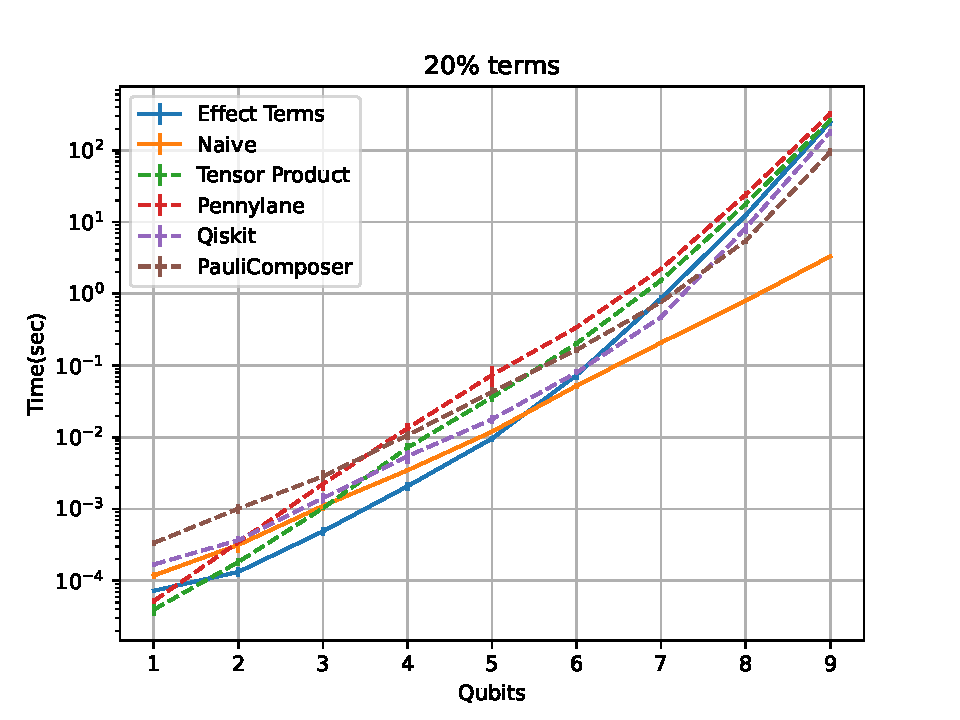
\includegraphics[width=0.5\linewidth]{0.2_terms.pdf}}
    \hfil
        \subfloat[]{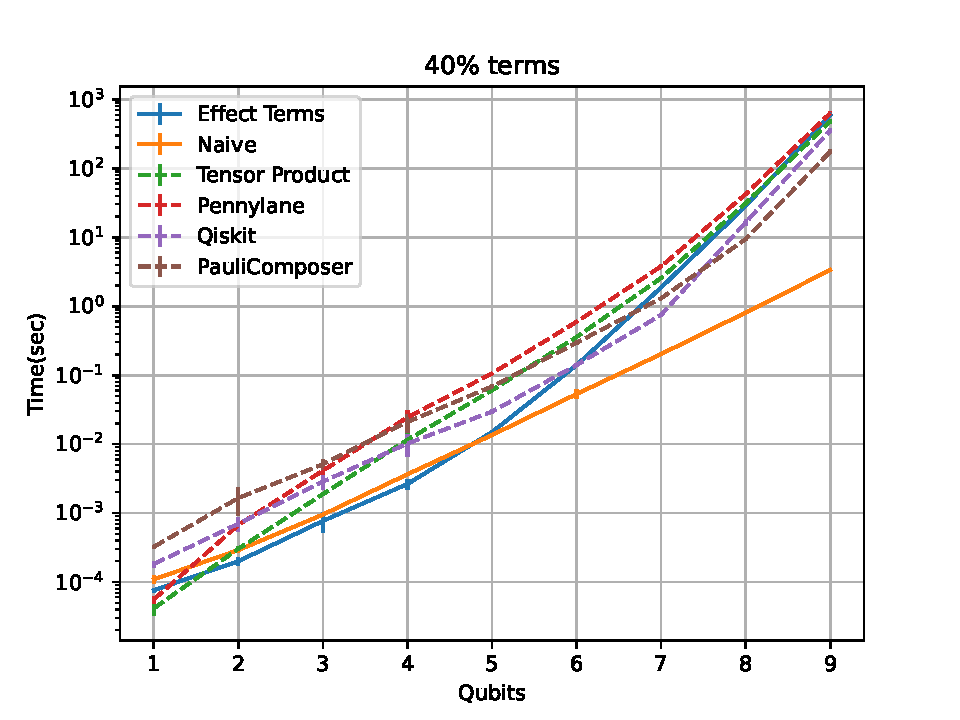
\includegraphics[width=0.5\linewidth]{0.4_terms.pdf}}
    
        \subfloat[]{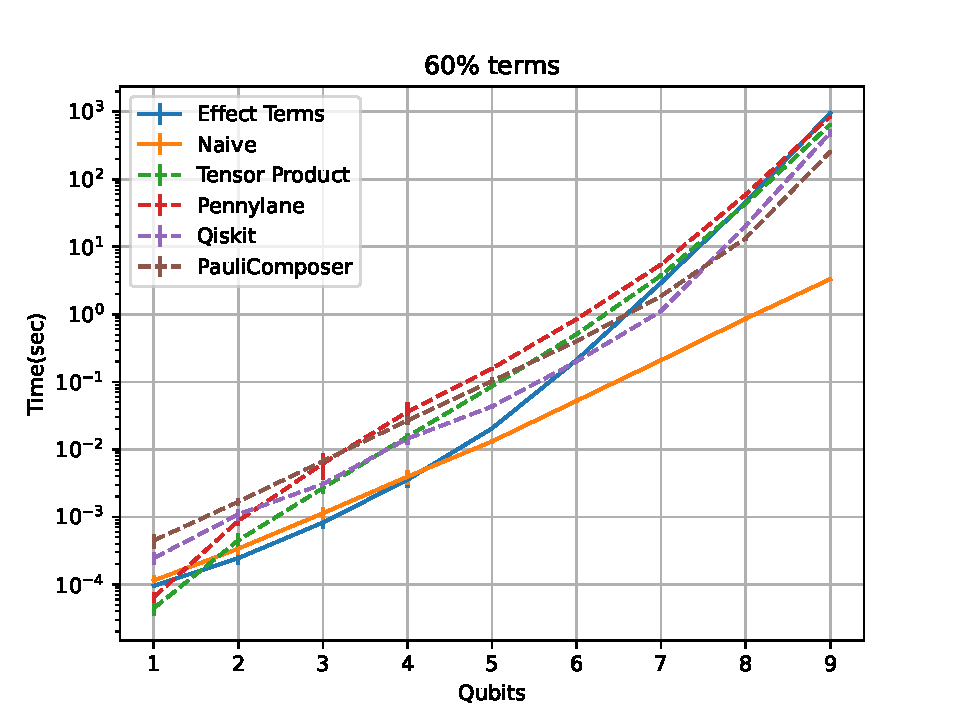
\includegraphics[width=0.5\linewidth]{0.6_terms.pdf}}
    \hfil
        \subfloat[]{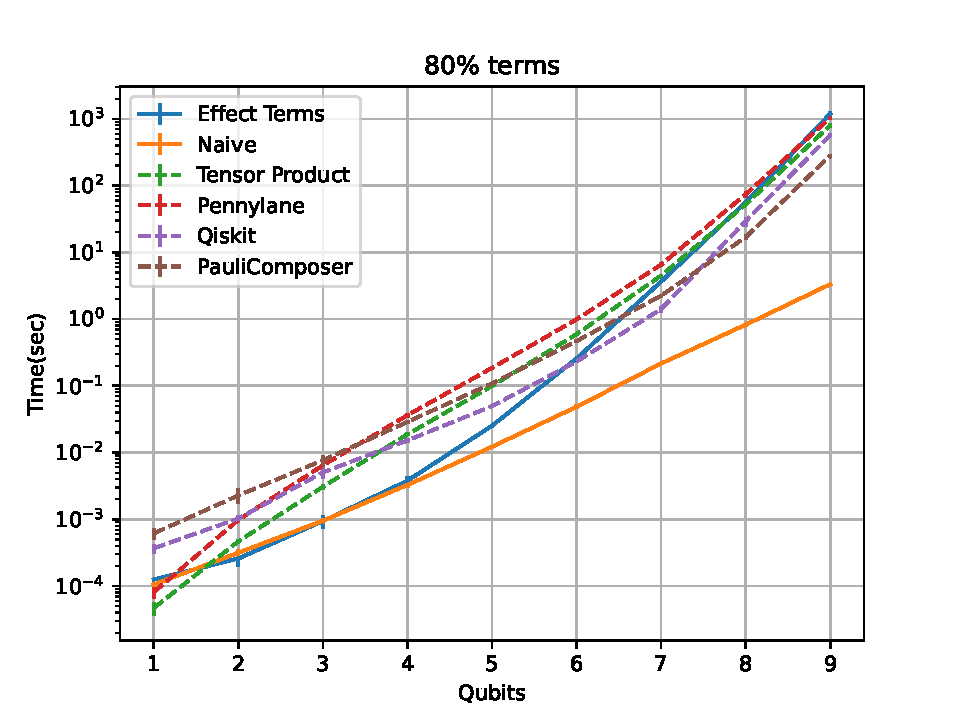
\includegraphics[width=0.5\linewidth]{0.8_terms.pdf}}
    
        \subfloat[]{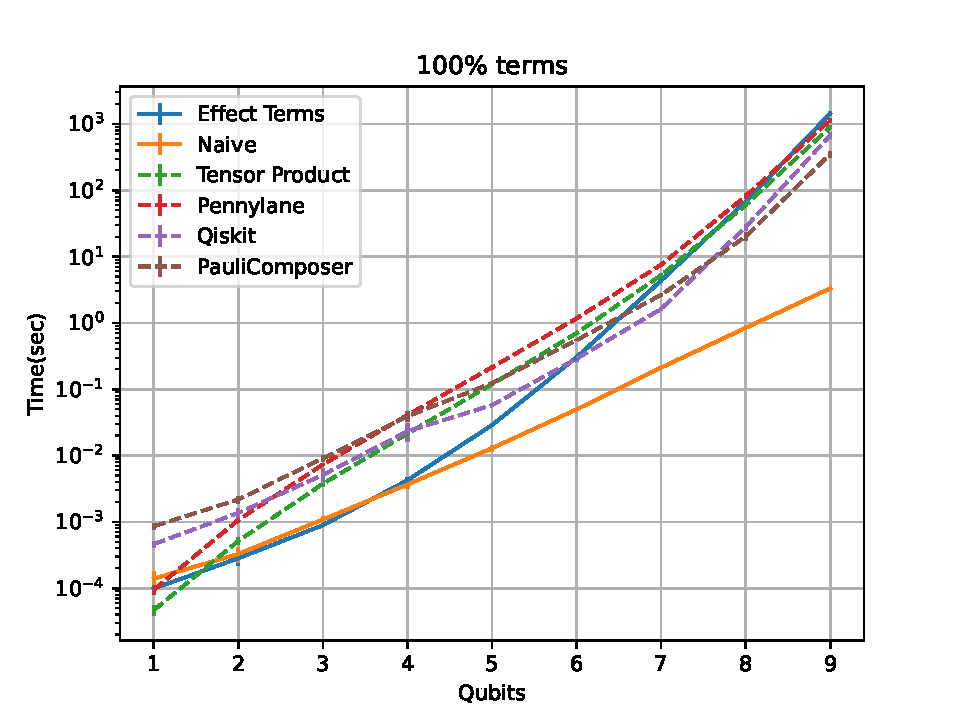
\includegraphics[width=0.5\linewidth]{1_terms.pdf}}
    \caption{Benchmarks for matrix composition of Puali polynomials with the algorithm \ref{alg:naive_inverse}, \ref{alg:effective_terms} with 
    Qiskit, Pennylane, PauliComposer, and standard tensor product methods, for $n=1$ to $n=9$. 
    The percentages of the each case represents how many coefficients are non-empty in $4^n$ number of spaces.}
        \label{fig:results}
\end{figure*}

\section{Conclusion}

In the paper, tensorized Pauli composition(\texttt{TPC}) algorithm was designed 
using a proper Pauli basis matrix and inverse Tensorizerd Pauli decomposition(\texttt{TPD}) algorithm\cite{Hantzko_2024}.
\texttt{TPD} was a sequential basis transformation of the given matrix.
The common XZ symplectic representation is one type of the transformation.
A simple conversion between the symplectic representation and an index of the Pauli basis matrix of \texttt{TPD}, 
was investigated and the inverse composition algorithms were designed.
Furthermore, a modified algorithm of \texttt{TPC} was designed by adding an effective term chasing routine.  
The chasing routine eliminates unnecessary terms in the naive \texttt{TPC} process,
so for sparse Pauli summation case, the algorithm is expected to show better result than naive version.

The algorithms are designed to compose the multiple terms simultaneously, thereby achieving better computational complexity in Pauli polynomial composition, in time and spatial both domains. 
The naive composition algorithm comprises a basis transformation mapping between the Pauli basis matrix and the original matrix representation.

Comparing to the previous term-by-term methods which have $O(16^n + 4^n(f(n)-1))$ complexity in the worst case, 
the naive algorithm is at least, twice faster than the common term-by-term methods  with $O(n4^n)$ complexity. 
It means that we can construct the matrix with computational basis corresponding to the given 
Pauli-polynomial at process of the algorithm. 
The inverse algorithm could chase effective terms during the composition process. 
However, the chasing routine incurs significant computational costs and is not as efficient as the naive version,
and even comparable with the term-by-term methods with $O(n16^n)$ complexity in the worst case.

In addition, the composition speed benchmark between the current quantum computing frameworks, Qiskit, Pennylane, and naive
tensor product routines. 
The inverse composition algorithm showed better speed for all cases, single, multi, worst terms 
for from $n=2$ to $n=9$ qubit cases. 
The naive algorithm was 10 or 1000 times faster than term-by-term methods.
Practically, even though the $k$ is small, the naive version is comparable 
with the term-by-term methods. 
We assume that it is caused from the spatial complexity effect.
The effective term algorithm could chase the effective terms, however in the current stage the time-cost benefit 
was not noticible in the implementation.

\section*{Acknowledgments}
The research was funded by the Quantum Sapiens Human Resources Center.

\section*{Data and code available}
The research was conducted for implementing a sub-module of OptTrot python package for 
fast manipulation and optimization routine for Hamiltonian.
OptTrot is a quantum computing frameworks for optimizing Trotter circuit on gate model computer.
The benchmarked code and data are on Github repository\cite{kim_2024_TPC}.
%Bibliography
\bibliographystyle{unsrt}  
\bibliography{references}  

\appendix
%\section{Basis choice of TPD}
%
%\subsection{Pauli operations with ij index}
%
%\textbf{Group addition}
%
%\begin{equation}
%    P_1 \cdot P_2 = P_3
%\end{equation}
%
%\begin{itemize}
%    \item $n_i^3 = n_i^2 {}^\wedge n_i^1$
%    \item $n_j^3 = n_j^2 {}^\wedge n_j^1$
%\end{itemize}
%\textbf{Tensor Product}
%
%\begin{equation}
%    P_1 \otimes P_2 = P_3
%\end{equation}
%\begin{itemize}
%    \item $n_i^3 = (2^m n_i^2) \vee n_i^1$
%    \item $n_j^3 = (2^m n_j^2) \vee n_j^1$
%\end{itemize}

\section{Computational aspects}
In real implementation, the chasing the efficient calculation term during 
the algorithm requires huge time complexity.
The current implementation use bitwise operation, since, Python is not good for 
manipulate binary data, efficiently\footnote{Bitwise operators are even slower than string manipulation in Python.}. 
The above routines would be more appropriate for C/C++ or Rust like language implementation.
We could observe that the binary compiled routines did not show difference 
whether the algorithm has a effective term chasing routine or not.
In python or the other interpreter language, it is wise to use the naive algorithm.
, and if the language environment naturally manipulate the bits, the effective term chasing version
would be more appropriate.

%\end{multicols*}
\end{document}
